% !TEX encoding = UTF-8 Unicode
% !TEX program = xelatexmk
% !TEX pdfSinglePage
\documentclass[12pt]{article}
%% Versioning info
%\usepackage[draft]{gitinfo2}
%% Polices OTF
\usepackage[libertine,libaltvw,liby,vvarbb]{newtxmath}
\usepackage[ttscale=.875]{libertine}
%\setmainfont{Lucida Grande}
%% Gestion des langues
\usepackage{polyglossia}
\setdefaultlanguage{english}
\usepackage[autostyle]{csquotes}
\MakeOuterQuote{"}
%% URLs and hyperlinks
\usepackage{xcolor}
\usepackage[unicode,bookmarks,colorlinks,breaklinks]{hyperref}
\hypersetup{linkcolor=blue,citecolor=blue,filecolor=blue,urlcolor=blue}
\urlstyle{same}
\usepackage[shortlabels]{enumitem}
%\setlist[enumerate,1]{label=\arabic*., ref=\arabic*}
%\setlist[itemize,1]{label=--,topsep=0pt,itemsep=0pt,leftmargin=*}
\setlist[itemize,1]{topsep=0pt,itemsep=0pt,leftmargin=1em}
\setlist[itemize,2]{topsep=0pt,itemsep=0pt}
%% Framed boxes
\usepackage[framemethod=tikz]{mdframed}
\global\mdfdefinestyle{verif}{%
  %linecolor=blue,middlelinewidth=2pt,
  roundcorner=5pt,
  frametitlebackgroundcolor=yellow!50!white,
}
\newmdenv[style=verif,frametitle=Check]{verification}
%% Format de page
\usepackage{geometry}
\geometry{a4paper}
\geometry{top=25mm, bottom=30mm}
\geometry{outer=22.5mm, inner=25mm}
\geometry{foot=15mm, head=15pt}
%% Paragraphes sans indentation, légèrement espacés
\setlength{\parindent}{0pt}
\setlength{\parskip}{3pt plus2pt minus1pt}
%%
\setcounter{tocdepth}{2}
\setcounter{secnumdepth}{1}
%%
\usepackage{listings}
\lstset{%
  basicstyle=\small\ttfamily,breaklines=true,
  showstringspaces=false,
  aboveskip=2\parskip,
  commentstyle=\color{darkgray},
  keywordstyle=\color[HTML]{000000},
  backgroundcolor=\color[HTML]{dddddd},
  tabsize=4,
  xleftmargin=1em,
  framextopmargin=3pt,
  framexleftmargin=1em,
  %framexrightmargin=1em,
  framexbottommargin=2pt,
  frame=bt,
  rulecolor=\color[HTML]{666666},
}
%%
%% Illustrations
\usepackage{graphicx}
\graphicspath{{img/}}

\begin{document}

\title{MoodleBox building reference\footnote{This work is licensed under a \href{http://creativecommons.org/licenses/by-nc-sa/4.0/}{Creative Commons Attribution - Non Commercial - Share Alike  4.0 International} license.}\\
Version 2.0 dev\footnote{This is work in progress, do not use!}}
\date{\today} %% \footnote{Version \gitAbbrevHash, \gitAuthorDate}
\author{Nicolas Martignoni}
\maketitle

\begingroup
\setlength{\parskip}{0pt}
\tableofcontents
\endgroup
\clearpage

\section{Introduction}

This article documents how to build a MoodleBox.
It is intended for developers or system administrators to provide background information on how a MoodleBox is built.

This is not meant to be an end-user documentation.
For end-user documentation, please consult \href{https://moodlebox.net/}{MoodleBox website}.

\subsection{Caveat}

The actual build of the MoodleBox image is done using \href{https://www.ansible.com/}{Ansible}.
Using Ansible enables most of the build to be automated, as well as ensuring that it is reproducible.
Though complete, the instructions in this document should not be understood as a method to obtain a MoodleBox that is totally equivalent to the officially published MoodleBox images.

\subsection{What MoodleBox does}

\begin{itemize}
\item Configurable routed wireless access point.
\item Internet router: If MoodleBox is connected via ethernet or wireless LAN to an Internet-connected network, it acts as a router and gives its clients access to the Internet.
\item DHCP server for wireless clients.
\item Moodle server (\url{http://moodlebox.home/}).
This is a fully standard Moodle installation.
\item MoodleBox plugin\footnote{\url{https://github.com/moodlebox/moodle-tool_moodlebox}.} providing a GUI to manage most aspects of the MoodleBox.
\end{itemize}

\subsubsection{Specific Moodle features}
\begin{itemize}
\item Moodle version 4.0.x in its basic configuration, with no content (no courses).
The only Moodle user account is an administrator account (username: \emph{moodlebox}, password: \emph{Moodlebox4\$}).
The server is configured to accept clients from the official Moodle app.\footnote{\url{https://download.moodle.org/mobile/}.} The \textsl{cron} service is launched every minute.
\item When a USB stick is inserted into the MoodleBox, its files are available to users in Moodle's \textsl{File system} repository.
\item Ability to upload files via SFTP directly to the MoodleBox; these files are then available to users in Moodle's \textsl{File system} repository.
\item Adminer, a full-featured database management tool, is installed (\url{http://moodlebox.home/adminer.php}).
\end{itemize}

\subsection{What MoodleBox doesn't do}

\begin{itemize}
\item Email server: MoodleBox is intended to be used "in the field", independently of any network infrastructure; email server functionality is not relevant for this purpose.
\item Coffee machine.
\end{itemize}

\section{Preparation of the Raspberry Pi}

Although the MoodleBox works fine on other models Raspberry Pi models, a Raspberry Pi Model 3B, 3B+ or 4B is recommended to \textbf{build} it.

\subsection{Copy of Raspberry Pi OS Lite on a microSD card}

We download the current version of \emph{Raspberry Pi OS Lite (64-bit)} from the Raspberry Pi web site,\footnote{\url{https://www.raspberrypi.com/software/operating-systems}.} and copy it on a (good quality!) microSD card.
A complete description of the process is available on Raspberry Pi web site.\footnote{See \url{https://www.raspberrypi.org/documentation/computers/getting-started.html}.}

We then insert the SD card into a computer and mount it.

\subsection{SSH access enabling}

For security reasons, SSH access isn't enabled by default in Raspberry Pi OS.
We must enable it, and to do so we create a file with name \lstinline{ssh.txt} in the boot partition of the microSD card; this is the part of the SD card which can be seen when it is mounted in a macOS or Windows computer.
The content of the file \lstinline{ssh.txt} doesn't matter.
The following commands will do this.

\begin{lstlisting}[language=bash]
$ cd <mounting point of "boot" partition>
$ touch ssh.txt
\end{lstlisting}

\subsection{Configuration of the main user account}\label{ssec-new-account}

For security reasons (again), the default image of Raspberry Pi OS Lite has no user account defined.
We need to create one, by adding a file \lstinline{userconf.txt} in the boot partition of the microSD card.
The MoodleBox image uses for this account the username \emph{moodlebox} and the password \emph{Moodlebox4\$}.

This file should contain a single line of text, consisting of \lstinline{username:password}: so the desired username, followed immediately by a colon, followed immediately by an \textbf{encrypted} representation of the password to use.\footnote{See \url{https://www.raspberrypi.com/documentation/computers/configuration.html}.}

\subsection{First login via SSH}

Eject the microSD card from the computer and insert it into the Raspberry Pi.

Connect the power supply of the Raspberry Pi.
Plug the Raspberry Pi with an Ethernet cable into a network with a DHCP server and wait 20-30 seconds.
The Raspberry Pi is now reachable on the network using the address \lstinline{raspberrypi.local}.\footnote{This network address is provided by the \emph{zeroconf} standard protocol.
Some older Android and Windows devices do not understand this protocol.
With such devices, it is necessary to get access to the Raspberry Pi via its numerical IP address, which must be discovered manually.}

\iffalse
\begin{verification}
Red LED, indicating the presence of power, lights up constantly.
Green LED, indicating accesses to the microSD card, flashes irregularly after 1-2 seconds.
\end{verification}
\fi

\iffalse
\begin{verification}
From a computer, we type the command \lstinline{ping -c3 raspberrypi.local}.
The result should be something like the following.

\begin{lstlisting}[language=bash]
$ ping -c3 raspberrypi.local
PING raspberrypi.local (192.168.1.212): 56 data bytes
64 bytes from 192.168.1.212: icmp_seq=0 ttl=64 time=0.452 ms
64 bytes from 192.168.1.212: icmp_seq=1 ttl=64 time=0.251 ms
64 bytes from 192.168.1.212: icmp_seq=2 ttl=64 time=0.222 ms

--- raspberrypi.local ping statistics ---
3 packets transmitted, 3 packets received, 0.0% packet loss
round-trip min/avg/max/stddev = 0.222/0.308/0.452/0.102 ms
\end{lstlisting}
\end{verification}
\fi

From now on, all operations are done via the command line, using \lstinline{ssh} (a regular terminal on macOS and Linux, or \lstinline{Putty} on Windows).

We can now log in to the Raspberry Pi using the main account we've just setup: username is \emph{moodlebox} with password \emph{Moodlebox4\$}.

\begin{lstlisting}[language=bash]
$ ssh moodlebox@raspberrypi.local
$ moodlebox@raspberrypi.local's password:
\end{lstlisting}

\iffalse
\begin{verification}
If all goes well, we are connected to the MoodleBox and the console displays

\begin{lstlisting}[language=bash]
The programs included with the Debian GNU/Linux system are free software;
the exact distribution terms for each program are described in the
individual files in /usr/share/doc/*/copyright.

Debian GNU/Linux comes with ABSOLUTELY NO WARRANTY, to the extent
permitted by applicable law.

moodlebox@raspberrypi:~ $
\end{lstlisting}
\end{verification}
\fi

\subsection{Raspberry Pi OS upgrade}

We begin by upgrading the Raspberry Pi's operating system and its installed packages, with these commands:
\begin{lstlisting}[language=bash]
$ sudo apt-get update -y
$ sudo apt-get full-upgrade -y
\end{lstlisting}

This step can take several minutes, depending on the available Internet connection speed.
We just wait until it's finished.

\subsection{Configuration of important settings}

Launch \emph{raspi-config} utility:
\begin{lstlisting}[language=bash]
$ sudo raspi-config
\end{lstlisting}

With \emph{raspi-config} utility, we configure the following settings.
\begin{itemize}
\item Expand Filesystem.
\item Install following \emph{locales}:
\begin{itemize}
\item \lstinline{de_DE.UTF-8}
\item \lstinline{en_AU.UTF-8}
\item \lstinline{en_GB.UTF-8}
\item \lstinline{es_ES.UTF-8}
\item \lstinline{fr_FR.UTF-8}
\item \lstinline{it_IT.UTF-8}
\end{itemize}
and set \lstinline{en_GB.UTF-8} as default \emph{locale}.
\item Set time zone and WLAN country.
This will also unblock wireless use.
MoodleBox default settings are respectively \lstinline{Europe/Zurich} and \lstinline{CH}.
\item Set the hostname to \emph{moodlebox}.
\end{itemize}

From now on, to connect to the Raspberry Pi (via SSH or SFTP), we'll use the address \lstinline{moodlebox.local}.

Let's reboot and log in to the MoodleBox with the default credentials set up page~\pageref{ssec-new-account}.

\subsection{Switch to the alternative wireless chip firmware}

The Raspberry Pi is usually used as a wireless client, and its wireless firmware has enhanced client features that are not useful for a MoodleBox, which is mainly used as an access point, not a wireless client.

However, the SRAM on the wireless chip is used both for data storage whilst in use, but also for these additional features and for bug fixes.
Each time a feature is added or a bug fix made, the amount of SRAM available for runtime variables decreases, and so the number of clients in access point mode.

An alternative firmware is now available that has been tuned to maximise the number of clients in access point mode (AP) while still supporting client mode (STA).
We want to use this alternative firmware in the MoodleBox.
To switch the firmware to the alternative one, we launch the following commands.

\begin{lstlisting}[language=bash]
$ cd /lib/firmware/brcm/
$ sudo ln -sf ../cypress/cyfmac43455-sdio-minimal.bin \
    brcmfmac43455-sdio.bin
\end{lstlisting}

\subsection{Raspberry Pi firmware upgrade  (optional)}

In very specific and very rare occasions, it's advisable to upgrade the firmware of the Raspberry Pi.
We only do this if we know why, since it could brick the device or the image!
And we reboot immediately.

\begin{lstlisting}[language=bash]
$ sudo apt-get install -y rpi-update
$ sudo SKIP_BACKUP=1 PRUNE_MODULES=1 rpi-update
$ sudo apt-get remove rpi-update
$ sudo reboot
\end{lstlisting}

\subsection{Configuration of the system memory}

To increase the system available memory, we reduce the memory reserved for the graphics chip to 16~MB.
This is of no consequence, as our system does have no graphical interface.
We do this by adding the following line at the end of the file \lstinline{/boot/config.txt}:
\begin{lstlisting}[language=bash]
gpu_mem=16
\end{lstlisting}

\subsection{Configuration of the shutdown/startup hardware button feature}

We enable shutdown/startup hardware button feature by further editing file \lstinline{/boot/config.txt}.
Insert following line after line beginning with \lstinline{# Additional overlays} to get:
\begin{lstlisting}[language=bash]
# Additional overlays and parameters are documented /boot/overlays/README
dtoverlay=gpio-shutdown
\end{lstlisting}

\section{Wireless access point feature}

We will now setup the wireless access point (AP) of the MoodleBox.

\subsection{Configuration of the wireless interface for access point mode}

We want to be able to use standard wireless interface \lstinline{wlan0} to optionally connect to a wireless LAN, so we need another interface for our AP.

We use a \textsl{udev} rule to define this new interface, creating a file named \lstinline{90-wireless.rules} in directory \lstinline{/etc/udev/rules.d/}.

Here's the content of \lstinline{/etc/udev/rules.d/90-wireless.rules} on the MoodleBox:
\lstinputlisting{files/90-wireless.rules}

%:TODO: Disable unused wpa_supplicant service?

\subsection{Configuration of the wireless connection as a client (optional)}

If MoodleBox is intended to be used as a client (STA mode) as well as an access point, a valid configuration file named \lstinline{wpa_supplicant.conf} should be provided to \lstinline{wpa_supplicant} service, in directory \lstinline{/etc/wpa_supplicant/}.

Following listing shows an example of such file:
\lstinputlisting{files/wpa_supplicant.conf}

Obviously the file should be edited to enter the real SSID and password of an existent wireless network.

\subsection{Installation of the packages for the access point feature}

The AP feature requires the packages \lstinline{hostapd} and \lstinline{dnsmasq}.
Let's install them.
\begin{lstlisting}[language=bash]
$ sudo apt-get install -y hostapd dnsmasq
\end{lstlisting}

\subsection{Configuration of the static IP address}\label{ssec-static-ip}

MoodleBox gets dynamically via DHCP its IP address on the ethernet interface \lstinline{eth0} or as a wireless client on the \lstinline{wlan0} interface.

With its routed access point feature, it will also act as a DHCP provider on its wireless interface \lstinline{uap0}, so we need a static IP address on \lstinline{uap0} interface. For the MoodleBox, we choose \lstinline{10.0.0.1}.
Any other private IP address can alternatively be used.

At the very end of file \lstinline{/etc/dhcpcd.conf}, we add the lines
\begin{lstlisting}[language=bash]
interface wlan0
# Uncomment following line to disable AP+STA mode
# nohook wpa_supplicant

interface uap0
static ip_address=10.0.0.1/24
nohook wpa_supplicant
\end{lstlisting}

\subsection{Configuration of the access point}

We can now configure the access point, by editing the file \lstinline{/etc/hostapd/hostapd.conf}.
This is where the access point SSID and password are set, as well as other options, such as the broadcast channel and regulatory country.
We define \emph{MoodleBox} as the SSID and \emph{moodlebox} as the password.

Here's the content of \lstinline{/etc/hostapd/hostapd.conf} on the MoodleBox:

\lstinputlisting[language=bash]{files/hostapd.conf}

\iffalse
\begin{verification}
Start \lstinline{hostapd}:
\begin{lstlisting}[language=bash]
$ sudo /usr/sbin/hostapd /etc/hostapd/hostapd.conf
\end{lstlisting}

We get an error message (expected as the configuration is not finished yet); this message should end with \lstinline{uap0: AP-ENABLED}.
Wireless clients should detect \emph{MoodleBox} SSID, even if they cannot to it.
\end{verification}
\fi

%:TODO: This was deprecated as of Bullseye and will be changed. 
% See /usr/share/doc/hostapd/README.Debian.

We now need to define where \lstinline{hostapd} gets its configuration.
This is set in file \lstinline{/etc/default/hostapd}, where we replace the line \lstinline{#DAEMON_CONF=""} with \lstinline{DAEMON_CONF="/etc/hostapd/hostapd.conf"}.
It should then have the following line:
\begin{lstlisting}[language=bash]
...
DAEMON_CONF="/etc/hostapd/hostapd.conf"
...
\end{lstlisting}

\iffalse
Here's the content of \lstinline{/etc/default/hostapd} after the substitution:
\lstinputlisting[language=bash]{files/hostapd}
\fi

Finally, we unmask and enable \lstinline{hostapd} service:
\begin{lstlisting}[language=bash]
$ sudo systemctl unmask hostapd
$ sudo systemctl enable hostapd
\end{lstlisting}

\subsection{Configuration of the DHCP and DNS server}

The DHCP and DNS server configuration on \lstinline{uap0} interface is provided through \lstinline{dnsmasq}.
%\footnote{DNS configuration is based on \url{https://www.linux.com/learn/dnsmasq-easy-lan-name-services}.}
We edit \lstinline{/etc/dnsmasq.conf} to have this content, where one notes the static IP address we set up on page~\pageref{ssec-static-ip}:

\lstinputlisting[language=bash]{files/dnsmasq.conf}

We edit now the file \lstinline{/etc/hosts}, replacing the last line, beginning with \lstinline{127.0.1.1}, with the following, containing the same static IP address defined earlier:
\begin{lstlisting}[language=bash]
10.0.0.1	moodlebox
\end{lstlisting}
This configuration enables any device to access the MoodleBox via its URL \url{http://moodlebox.home/}, even those that do not implement \emph{zeroconf}\footnote{\url{https://en.wikipedia.org/wiki/Zero-configuration_networking}} standard protocol.

Finally, we fix a race condition between \lstinline{dhcpcd} and \lstinline{dnsmasq} by editing \lstinline{dnsmasq} service file \lstinline{/lib/systemd/system/dnsmasq.service}.
We add following lines just before \lstinline{[Install]}:
\begin{lstlisting}[language=bash]
RestartSec=5
Restart=on-failure
\end{lstlisting}

\subsection{Configuration of mDNS services advertising}

In order to make MoodleBox services visible on the network, we create the file \lstinline{/etc/avahi/services/moodlebox.service}, with following content.
\lstinputlisting[language=xml]{files/moodlebox.service.xml}

\subsection{Routing configuration}

We configure now the routing, so that the wireless clients can browse the Internet when MoodleBox is connected to an Internet router (via ethernet or wireless).

We edit the file \lstinline{/etc/sysctl.conf}, uncommenting or adding the line
\begin{lstlisting}[language=bash]
net.ipv4.ip_forward=1
\end{lstlisting}

The installation of the package \lstinline{iptables-persistent} enables routing rules to survive MoodleBox reboot or shutdown.
\begin{lstlisting}[language=bash]
$ sudo apt-get install -y iptables-persistent
\end{lstlisting}

We can now define the routing rules:
\begin{lstlisting}[language=bash]
$ sudo iptables -t nat -A POSTROUTING -o eth0 -j MASQUERADE
$ sudo iptables -t nat -A POSTROUTING -o wlan0 -j MASQUERADE
$ sudo iptables -A FORWARD -i eth0 -o uap0 \
    -m state --state RELATED,ESTABLISHED -j ACCEPT
$ sudo iptables -A FORWARD -i wlan0 -o uap0 \
    -m state --state RELATED,ESTABLISHED -j ACCEPT
$ sudo iptables -A FORWARD -i uap0 -o eth0 -j ACCEPT
$ sudo iptables -A FORWARD -i uap0 -o wlan0 -j ACCEPT
\end{lstlisting}

And we reboot.
\begin{lstlisting}[language=bash]
$ sudo reboot
\end{lstlisting}

\iffalse
\subsection{Wireless access point testing}

\begin{verification}
After rebooting, a client device should be able to browse Internet after connecting to the \emph{MoodleBox} Wi-Fi network with password \emph{moodlebox}.
\end{verification}
\fi

\subsection{Installation and configuration of the captive portal}

We can now install the captive portal, based on the free software Nodogsplash.\footnote{\url{https://nodogsplashdocs.readthedocs.io/}.}
Nodogsplash needs first to be compiled for the Raspberry Pi platform.
\href{https://nodogsplashdocs.readthedocs.io/en/stable/compile.html}{Nodogsplash documentation} gives info about its compilation, which is not covered in this guide.

Let's install the Nodogsplash package we got after compilation:
\begin{lstlisting}[language=bash]
$ sudo dpkg –i nodogsplash_5.0.0-1_armhf.deb
\end{lstlisting}
Nodogsplash configuration file \lstinline{/etc/nodogsplash/nodogsplash.conf} should read (note the static IP address defined earlier)
\lstinputlisting[language=bash]{files/nodogsplash.conf}

We can now edit Nodogsplash splash page at our convenience.
The files to edit are located in directory \lstinline{/etc/nodogsplash/htdocs/}.

In the official MoodleBox image, Nodogsplash captive portal is not enabled.
If we want to disable it too, we type following commands in our shell:
\begin{lstlisting}[language=bash]
$ sudo systemctl stop nodogsplash.service
$ sudo systemctl disable nodogsplash.service
\end{lstlisting}

\section{Installation of the LEMP stack}

The LEMP software stack is a group of software that can be used to serve dynamic web pages and web applications.
The term LEMP is an acronym that represents a Linux operating system with an Nginx (pronounced "engine-x", hence the E in the acronym) web server.
The backend data is stored in a MariaDB database and the dynamic processing is handled by PHP.

\subsection{Installation of Nginx and PHP}\label{ssec-nginx-php-installation}

We install first Nginx and all needed PHP packages, notably those required by Moodle.

\begin{lstlisting}[language=bash]
$ sudo apt-get install -y nginx php7.4-fpm php7.4-cli php7.4-common \
    php7.4-json php7.4-mbstring php7.4-opcache php7.4-readline \
    php7.4-xmlrpc php7.4-curl php7.4-gd php7.4-intl php7.4-soap \
    php7.4-mysql php7.4-xml php7.4-zip php7.4 php-apcu
\end{lstlisting}

\iffalse
\begin{verification}
With a computer connected to the MoodleBox wireless network, we load URL \url{http://moodlebox.home/} in a web browser.
The web page "Welcome to nginx on Debian!" Should be displayed.
\end{verification}
\fi

%:TODO: >--- pointer ---<

\subsection{SSL certificate and key}

We can now copy the SSL certificate \lstinline{moodlebox.pem} and its key \lstinline{moodlebox.key} to the directory \lstinline{/etc/nginx/}.

SSL certificate generation is not covered in this guide, but any help can be 
found in any adequate documentation on SSL certificate generation, e.g. on \url{https://stackoverflow.com/a/10176685}.

\subsection{Web server configuration: Nginx and PHP}

Nginx web server configuration is set in file \lstinline{/etc/nginx/sites-available/default}, which content should be like below.
\lstinputlisting[language=bash]{files/default}

Last \lstinline{fastcgi_param} line, with line \lstinline{client_max_body_size}, increases to 50~MB the max upload file size, as well as script maximum execution time to~300~s.
It also sets \lstinline{max_input_vars} to~5000.

We then relaunch the web server:
\begin{lstlisting}[language=bash]
$ sudo systemctl restart nginx php7.4-fpm
\end{lstlisting}

\iffalse
\begin{verification}
We type the command
\begin{lstlisting}[language=bash]
$ echo '<?php phpinfo(); ?>' | sudo tee -a /var/www/html/info.php
\end{lstlisting}
then open URL \url{http://moodlebox.home/info.php} in a browser.
The long PHP settings page should appear, with the \lstinline{upload_max_filesize}, \lstinline{post_max_size} and \lstinline{max_input_vars} variables correctly set.
\end{verification}
\fi

The ownership, group and access rights of Nginx and PHP should now be tweaked so that the default user \emph{moodlebox} can easily edit the files, while allowing Moodle updates and plugin installation via the web interface.

To do this, we edit the two files \lstinline{/lib/systemd/system/nginx.service} and \lstinline{/lib/systemd/system/php7.4-fpm.service}, adding after line \lstinline{[Service]} the line \lstinline{UMask=0002}, to get something like
\begin{lstlisting}[language=bash]
...
[Service]
UMask=0002
Type=...
...
\end{lstlisting}
We then edit the file \lstinline{/etc/php/7.4/fpm/pool.d/www.conf} to set the correct group ownership for PHP, replacing line \lstinline{group = www-data} with \lstinline{group = moodlebox}, so we have now
\begin{lstlisting}[language=bash]
...
user = www-data
group = moodlebox
...
\end{lstlisting}
If needed, variables in \lstinline{/etc/php/7.4/fpm/pool.d/www.conf} can be tweaked, e.g. for performance gains. See section~\ref{sec-optimisation} for examples.

\subsection{MariaDB installation and configuration}

We install now MariaDB package.
PHP MariaDB support was already installed with PHP (see section~\ref{ssec-nginx-php-installation}).
\begin{lstlisting}[language=bash]
$ sudo apt-get install -y mariadb-server
\end{lstlisting}

During the installation, we define the password of the main user \emph{moodlebox} of the database.
For this installation, we set the password to \emph{Moodlebox4\$}.

\iffalse
\begin{verification}
Reload URL \url{http://moodlebox.home/info.php}.
A new section \emph{MySQL} should appear in the page.
\end{verification}
\fi

In order to allow flexible access to the databases, a new database user is created in MariaDB.

\begin{lstlisting}[language=bash]
$ sudo mysql
    > CREATE USER 'moodlebox'@'localhost' IDENTIFIED BY 'Moodlebox4$';
    > GRANT ALL PRIVILEGES ON *.* TO 'moodlebox'@'localhost';
    > FLUSH PRIVILEGES;
    > QUIT;
\end{lstlisting}

If needed, variables in \lstinline{/etc/mysql/mariadb.conf.d/50-server.cnf} can be tweaked, e.g. for performance gains. See section~\ref{sec-optimisation} for examples.

\section{Installation and configuration of Moodle}

\subsection{Moodle database creation}

We first create the database which Moodle will use.
\begin{lstlisting}[language=bash]
$ sudo mysql
    > CREATE DATABASE moodle;
    > QUIT;
\end{lstlisting}

\subsection{Moodle download}

We can now download Moodle; we do this with Git in order to facilitate future updates.
We first install Git.
\begin{lstlisting}[language=bash]
$ sudo apt-get install -y git
\end{lstlisting}

We get now Moodle source in the appropriate location, specifying the current stable branch of Moodle.
A shallow clone is used to later save space on the MoodleBox image.
\begin{lstlisting}[language=bash]
$ sudo git clone --depth=1 -b MOODLE_311_STABLE \
    git://git.moodle.org/moodle.git /var/www/moodle
\end{lstlisting}

%\subsection{Moodle configuration}
\subsection{Creation of Moodle data directories}

Moodle data and several other directories are now created.
\begin{lstlisting}[language=bash]
$ sudo mkdir -p /var/www/moodledata/repository /var/www/moodledata/temp \
    /var/www/moodledata/backup /var/cache/moodle \
    /var/cache/moodle-cache-backup
\end{lstlisting}
Adequate permissions and ownership are set on these directories, including SGID permission on Moodle data directory.
We also set the correct permissions to Moodle source directory:
\begin{lstlisting}[language=bash]
$ sudo chown -R www-data:moodlebox /var/www/moodle /var/www/moodledata/ \
    /var/cache/moodle /var/cache/moodle-cache-backup
$ sudo chmod -R ug+w,o-w /var/www/moodle /var/www/moodledata/ \
    /var/cache/moodle /var/cache/moodle-cache-backup
$ sudo chmod -R g+s /var/www/moodledata/
\end{lstlisting}

We can now launch Moodle installation, either by loading URL \url{http://moodlebox.home/} in a browser and follow the instructions on screen, or by using Moodle command line interface.\footnote{See \url{https://docs.moodle.org/311/en/Installing_Moodle\#Command_line_installer}.}
For MoodleBox, the administrator account is defined with \emph{moodlebox} as username and the password \emph{Moodlebox4\$}.

The installation takes at least 10 minutes.
Be patient!

\subsection{Tweaking the Moodle configuration}

\subsubsection{Moodle course backup directory}

As we use for Moodle course backup a different directory than the data directory, we set the following line in Moodle configuration file \lstinline{/var/www/moodle/config.php}:
%, just after line \lstinline{$CFG->admin = 'admin';}
\begin{lstlisting}[language=php]
$CFG->backuptempdir = '/var/www/moodledata/backup';
\end{lstlisting}

\subsubsection{\emph{X-Sendfile} setup}

We set \emph{X-Sendfile} in \lstinline{/var/www/moodle/config.php} to allow files in the Moodle data directory to be uploaded faster through the web server:
\begin{lstlisting}[language=php]
$CFG->xsendfile = 'X-Accel-Redirect';
$CFG->xsendfilealiases = array ('/dataroot/' => $CFG->dataroot);
\end{lstlisting}
For \emph{X-Sendfile} to be active, we must add following lines to Nginx configuration file \lstinline{/etc/nginx/sites-available/default}, inside \lstinline{server} block:
\begin{lstlisting}[language=bash]
location /dataroot/ {
    internal;
    alias /var/www/moodledata/;
}
\end{lstlisting}

\subsubsection{Custom filetype definition}

Defining a custom file type in Moodle facilitates the web certificate from MoodleBox home page. The definition is coded in \lstinline{/var/www/moodle/config.php} too:
\begin{lstlisting}[language=php]
$CFG->customfiletypes = array(
  (object)array(
    'extension' => 'crt',
    'icon' => 'sourcecode',
    'type' => 'application/x-x509-ca-cert',
    'customdescription' => 'X.509 CA certificate'
  )
);
\end{lstlisting}

\subsubsection{Hiding content that doesn't make sense for MoodleBox}

We hide Moodle campaign and Moodle services and support sections from notifications page.
These content don't make sense for MoodleBox, which is offline most of the time.
\begin{lstlisting}[language=php]
$CFG->showcampaigncontent = false;
$CFG->showservicesandsupportcontent = false;
\end{lstlisting}

Final content of the file \lstinline{/var/www/moodle/config.php} is then:
\lstinputlisting[language=php]{files/config.php}

%Final content of the file \lstinline{/etc/nginx/sites-available/default} is then:
%\lstinputlisting[language=bash]{files/default2}

\subsection{Cron configuration}

Moodle cron should be launched every minute.
Moreover, since MoodleBox is offline most of the time and doesn't have a mail server, no mail should be sent by cron process.
We edit cron configuration with the shell command
\begin{lstlisting}[language=bash]
$ sudo crontab -e
\end{lstlisting}
and add following lines to the crontab
\begin{lstlisting}[language=bash]
MAILTO=""
* * * * * nice -n10 /usr/bin/php /var/www/moodle/admin/cli/cron.php
\end{lstlisting}

\iffalse
\begin{verification}
Visit Moodle administration via \emph{Site administration > Server > Scheduled tasks}, check that the scheduled tasks are launched regularly.
\end{verification}
\fi

\section{MoodleBox plugin}

MoodleBox plugin\footnote{MoodleBox plugin source code is available at \url{https://github.com/moodlebox/moodle-tool_moodlebox}.} enables monitoring of the MoodleBox as well as managing several of its settings, such as password change, date and time setting, wireless access settings, etc.

This plugin works only on Raspberry Pi hardware, and needs some prerequisites to work

\subsection{Installation of the MoodleBox plugin in Moodle}

As usually, we install the plugin in Moodle by visiting \emph{Site administration > Plugins > Repositories > Install plugins}.
Click on the \emph{Install plugins from the Moodle plugins directory} button and select \emph{MoodleBox} administration plugin (\emph{Admin tools}).

It's also possible to install it via Git.

\begin{lstlisting}[language=bash]
$ cd /var/www/moodle/admin/tool/
$ sudo git clone https://github.com/moodlebox/moodle-tool_moodlebox.git moodlebox
\end{lstlisting}

In this case, we need to complete the installation of the plugin by visiting the page \url{http://moodlebox.home/admin}.

\subsection{Finalisation of the installation of the MoodleBox plugin}

To finalise the installation of the MoodleBox plugin, we need to create of a few files and set their permissions.
We'll also set the correct owner, group and permissions for all the plugin files.
\begin{lstlisting}[language=bash]
$ cd /var/www/moodle/admin/tool/moodlebox
$ sudo touch .reboot-server .shutdown-server .set-server-datetime \ 
    .newpassword .wifisettings .resize-partition
$ sudo chown -R www-data:moodlebox /var/www/moodle/admin/tool/moodlebox
$ sudo chmod -R ug+w,o-w /var/www/moodle/admin/tool/moodlebox
$ sudo chmod -R 774 /var/www/moodle/admin/tool/moodlebox/bin
\end{lstlisting}

We install \lstinline{direvent} and configure some jobs so that the MoodleBox plugin works correctly.
\begin{lstlisting}[language=bash]
$ sudo apt-get install -y direvent
\end{lstlisting}
Here's the configuration file of \lstinline{direvent}:
\lstinputlisting[language=bash]{files/direvent.conf}

Lastly, we copy these lines at the end of \lstinline{/etc/sudoers.d/020_www-data-nopasswd} (or create it if it's not there):
\lstinputlisting[language=bash]{files/020_www-data-nopasswd}

And we don't forget to reboot now!

\section{Moodle repositories for USB sticks and SFTP uploads}

Let's now configure the Moodle \textsl{File system} repositories, which will make it easier for MoodleBox's users to manage the files they want to provide with Moodle.

\subsection{USB sticks}

We set up automatic mounting of USB sticks (regardless of their format), as well as access to all files on inserted USB sticks via the \textsl{File system} repository.\footnote{If more than one USB stick is inserted into the MoodleBox, only the files on the first inserted stick are accessible via the File system repository.}

This is done by installing the \lstinline{usbmount} package, then creating a directory in the Moodle data directory, and finally creating a link from the USB stick mount point to this directory.

The \lstinline{usbmount} package should be built from its source code before to be installed.\footnote{See \url{https://github.com/rbrito/usbmount}. Follow the instructions in the README file.}
We also install standard packages to support exFAT and NTFS formatted devices. Support for other formats is built-in.

\begin{lstlisting}[language=bash]
$ sudo apt-get install -y ntfs-3g exfat-fuse
$ sudo dpkg –i usbmount_0.0.24_all.deb
$ sudo mkdir -p /var/www/moodledata/repository
$ sudo chown -R www-data:moodlebox /var/www/moodledata/
$ sudo ln -s /media/usb /var/www/moodledata/repository
\end{lstlisting}

We then have to configure Moodle appropriately:\footnote{See \url{https://docs.moodle.org/en/File_system_repository}.}
having logged in to Moodle as an administrator, visit \emph{Site administration > Plugins > Repositories > Manage repositories}.

Select \emph{Enabled and visible} in the row \emph{File system} to enable this repository.
\begin{figure}[!ht]
\begin{minipage}[b]{\linewidth}\centering
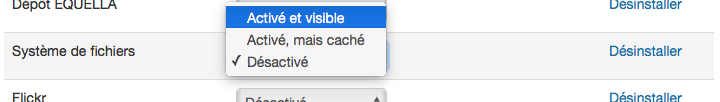
\includegraphics[width=13cm]{repo-filesystem-usb-1.png}
\end{minipage}
\end{figure}

Click on \emph{Save}.
Then, on the same row, click on \emph{Settings}, then on \emph{Create a repository instance}.
Finally select \emph{usb} from the drop-down menu, and enter \emph{USB Drive} in the mandatory \emph{Name} field.
\begin{figure}[!ht]
\begin{minipage}[b]{\linewidth}\centering
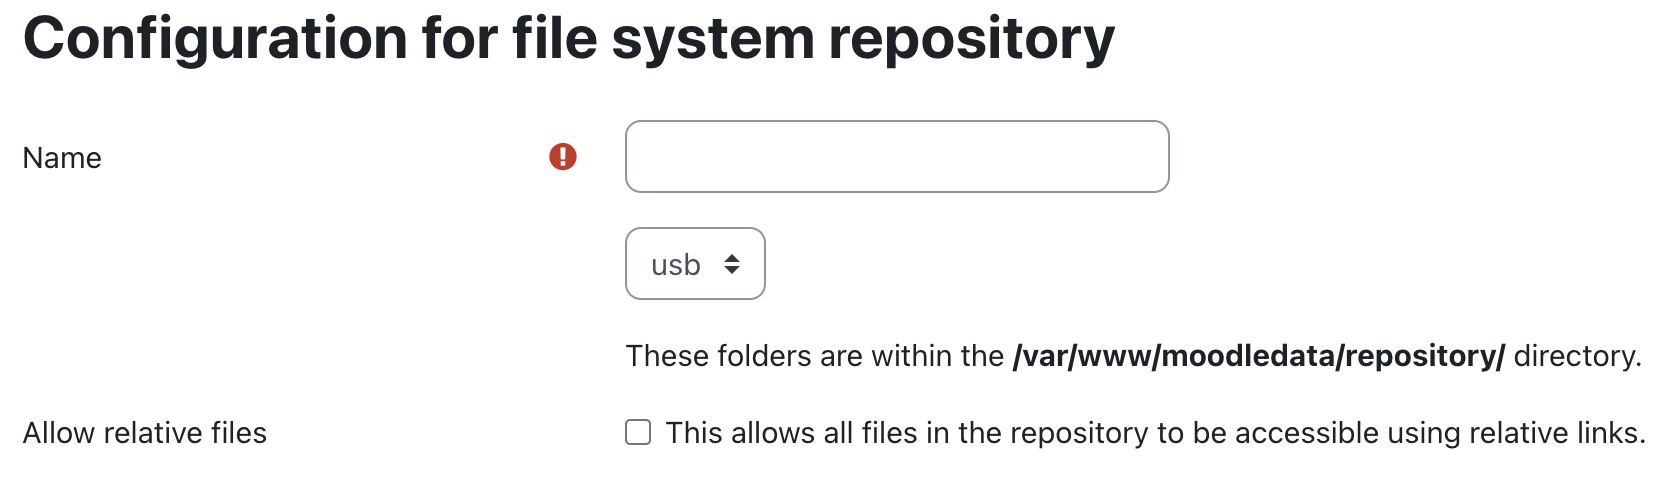
\includegraphics[width=13cm]{repo-filesystem-usb-2.png}
\end{minipage}
\end{figure}

\subsection{SFTP upload}

We create a directory in which the files will be dropped in order to be accessible from Moodle, as well as a link to the Moodle data directory.
Appropriate permissions are set.
\begin{lstlisting}[language=bash]
$ mkdir -p /home/moodlebox/files
$ sudo chown -R moodlebox:www-data files/
$ sudo chmod g+s files/
$ sudo ln -s /home/moodlebox/files /var/www/moodledata/repository
\end{lstlisting}

The repository is then configured in a similar way to the \textsl{USB Drive} repository above, by specifying the directory \emph{files} and enter \emph{SFTP Documents} as the repository name.

To use this feature, MoodleBox's admin will log in to the MoodleBox using a SFTP software\footnote{For instance: \href{https://filezilla-project.org/}{FileZilla}, \href{https://cyberduck.io/}{Cyberduck}, \href{http://winscp.net/}{WinSCP}.}, with the user name \emph{moodlebox} and the password \emph{Moodlebox4\$}.
He can then upload files in the \lstinline{files} directory.

\section{Additional Moodle configurations}

\subsection{Enabling access to the MoodleBox via the Moodle mobile app}

After logging in to Moodle with the administrator account, we visit \textsl{Site Administration > Advanced features}.
We check the box \emph{Enable web services for mobile devices} and save the changes.

For MoodleBox, which is not intended to be published on the Internet, the warning\footnote{Text of the warning: \textsl{It is recommended to enable HTTPS with a valid certificate. The Moodle app will always try to use a secured connection first}.} about the SSL certificate can be safely ignored.

\iffalse
\begin{verification}
From a smartphone connected to the MoodleBox network via Wi-Fi, launch the Moodle mobile app and connect to the platform using the URL \url{http://moodlebox.home}, with the administrator account.
No errors should be notified, and the dashboard should be displayed on the smartphone screen.
\end{verification}
\fi

\subsection{Utilities to use PDF files in Moodle}

We install Ghostscript and Poppler to enable Moodle to manage PDF annotations and PDF to PNG conversions.
\begin{lstlisting}[language=bash]
$ sudo apt-get install -y ghostscript poppler-utils
\end{lstlisting}

\section{Installation of \textsl{Adminer}}

\textsl{Adminer} is a full-featured database management tool written in PHP. It consists of a single file ready to be deployed to the server.
We install it by downloading it to the adequate location, and set its appropriate permissions.
\begin{lstlisting}[language=bash]
$ cd /var/www/moodle/
$ sudo wget -c https://www.adminer.org/latest.php -O adminer.php
$ sudo chown moodlebox:www-data adminer.php
$ sudo chmod -R 664 adminer.php
\end{lstlisting}

To manage the database with \textsl{Adminer}, the interface should be accessed at \url{http://moodlebox.home/adminer.php}.
To log in, use usual credentials: by default, username \emph{moodlebox} and password \emph{Moodlebox4\$}.

\iffalse
\begin{verification}
Browse to URL \url{http://moodlebox.home/adminer.php}.
The Adminer interface should be displayed.
To log in, use usual credentials: by default, username \emph{moodlebox} and password \emph{Moodlebox4\$}.
\end{verification}
\fi

\section{Optimisation}\label{sec-optimisation}

To make the MoodleBox more comfortable to use, it is necessary to take care of its optimisation.
We configure Moodle's cache, as well as its management of file uploads and downloads.

\subsection[RAM disks for some Moodle directories]{RAM disks for some Moodle directories\footnote{Inspired by \url{https://www.leading-interactive.de/e-learning/moodle-performance-tuning-mit-tmpfs/}.}}

Some files in Moodle data directory are needed very frequently.
To enable faster access to them, we deliver them directly from the server's RAM, faster than the SD-card.

We create a directory as a mount point for the RAM disk, with adequate permissions.
This directory will contain the cache files that we will define below. 
\begin{lstlisting}[language=bash]
$ sudo mkdir /var/cache/moodle
$ sudo chown www-data:moodlebox /var/cache/moodle/
$ sudo chmod ug+w,o-w /var/cache/moodle/
\end{lstlisting}

RAM disks are also used for the temporary and sessions directories in Moodle.
These two directories are located Moodle data directory \emph{moodledata}.

We define the RAM disks in the Raspberry's mount table.
To do this, we add the following lines to the file \lstinline{/etc/fstab}:
\begin{lstlisting}[language=bash]
tmpfs /var/cache/moodle tmpfs size=64M,mode=775,uid=www-data,gid=www-data 0 0
tmpfs /var/www/moodledata/temp tmpfs size=64M,mode=775,uid=www-data,gid=www-data 0 0
tmpfs /var/www/moodledata/sessions tmpfs size=16M,mode=775,uid=www-data,gid=www-data 0 0
\end{lstlisting}

%\begin{lstlisting}[language=bash]
%$ sudo nano /etc/fstab
%\end{lstlisting}
%
%Le contenu du fichier \lstinline{/etc/fstab} sera alors :
%\lstinputlisting[language=bash]{files/fstab}

After a reboot of the MoodleBox, the cache can be configured in Moodle.

Log in to Moodle with the administrator account, then visit \textsl{Site Administration > Plugins > Caching > Configuration}.
We create two new cache stores, by clicking on \emph{Add Instance} in the \emph{Installed cache stores} section (at the top of the page).

\begin{figure}[!ht]
\hspace{\fill}
\begin{minipage}[b]{0.45\linewidth} % A minipage that covers half the page
\centering
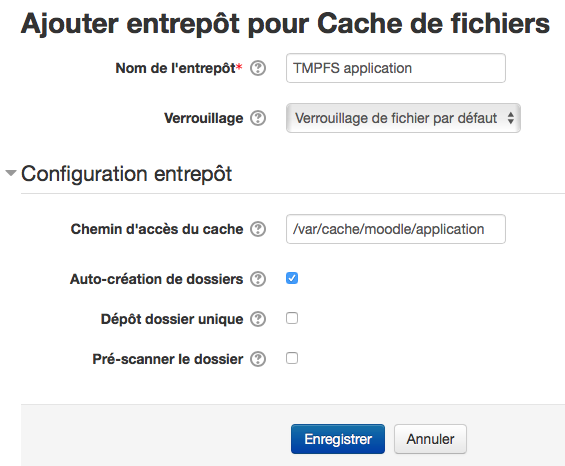
\includegraphics[width=7.3cm]{cache-application.png}
\end{minipage}
\hspace{\fill} % To get a little bit of space between the figures
\begin{minipage}[b]{0.45\linewidth}
\centering
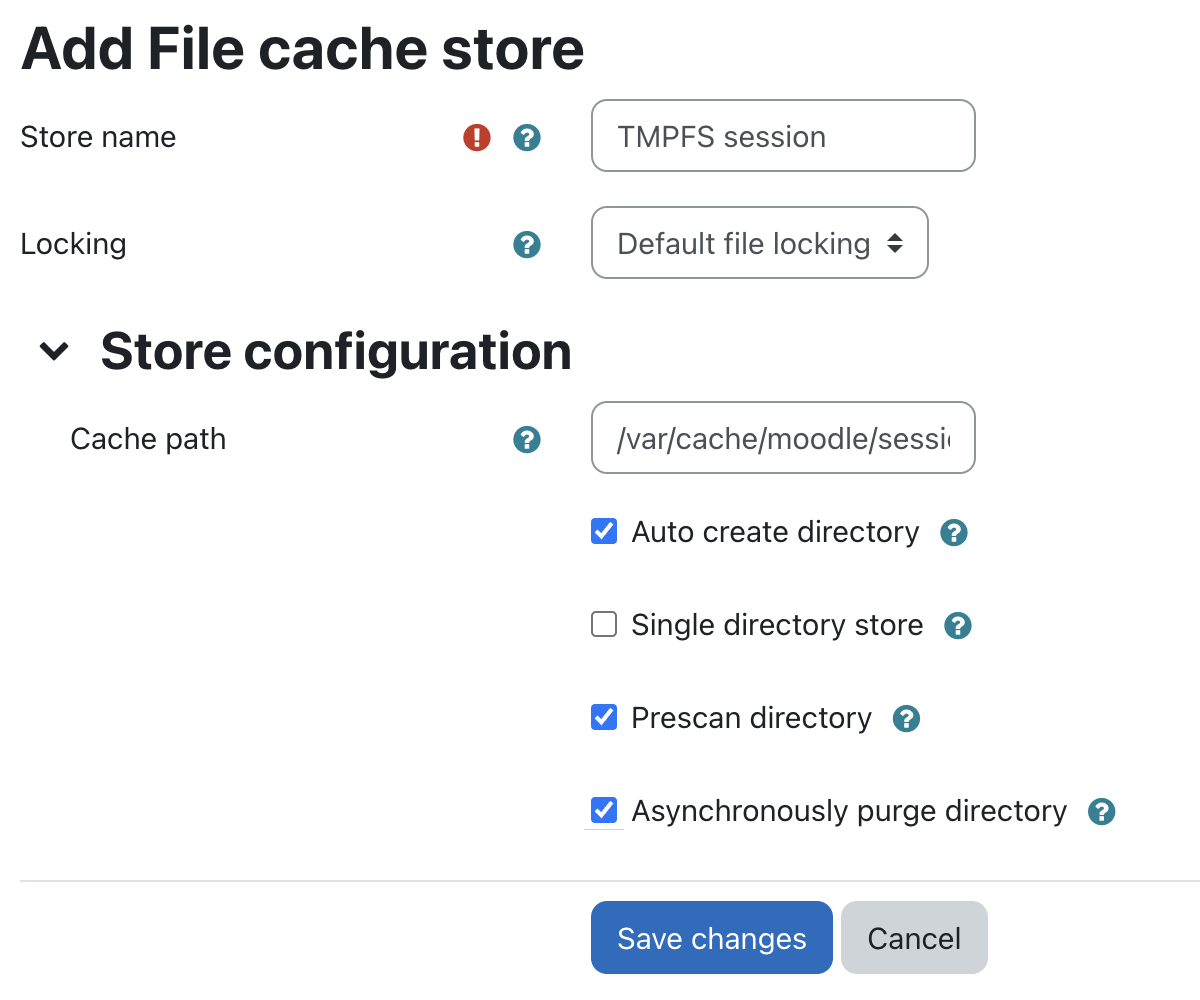
\includegraphics[width=7.3cm]{cache-session.png}
\end{minipage}
\hspace{\fill}
\end{figure}

\begin{enumerate}
\item Store name: \emph{TMPFS application}, Cache path: \emph{/var/cache/moodle/application}, check the boxes \emph{Auto create directory}, \emph{Prescan directory} and \emph{Asynchronously purge directory};
\item Store name: \emph{TMPFS session}, Cache path: \emph{/var/cache/moodle/session}, check the boxes \emph{Auto create directory}, \emph{Prescan directory} and \emph{Asynchronously purge directory}.
\end{enumerate}

Finally, we map these new cache instances with their destination, by clicking on \emph{Edit mappings} in the \emph{Stores used when no mapping is present} section, at the very bottom of the page.

\begin{figure}[!ht]
\begin{minipage}[b]{\linewidth}
\centering
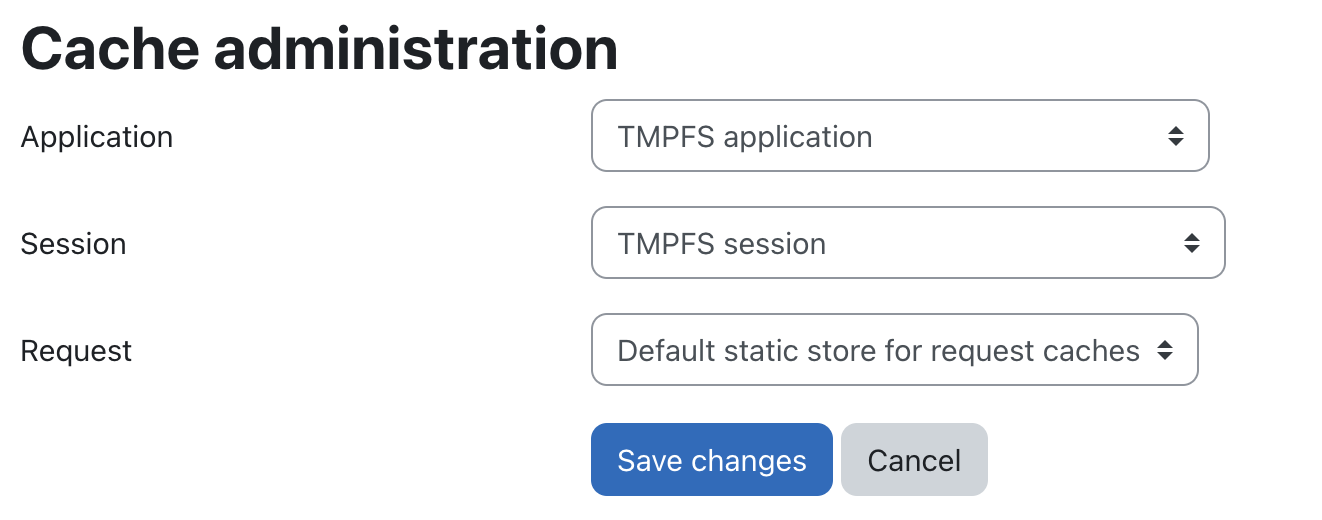
\includegraphics[width=11cm]{cache-mappings.png}
\end{minipage}
\end{figure}

\iffalse
\begin{verification}
After some actions on the Moodle platform of the MoodleBox, connect via SSH to the MoodleBox, then run the command
\begin{lstlisting}[language=bash]
ls -l /var/cache/moodle/
\end{lstlisting}
The console should display something like
\begin{lstlisting}[language=bash]
total 0
drwxrwxrwx 59 www-data moodlebox 1180 Oct  9 21:41 application
drwxrwxrwx 13 www-data moodlebox  260 Oct  9 21:41 session
\end{lstlisting}
\end{verification}
\fi

Putting the cache in a RAM disk has one big drawback: the data in it disappears every time the MoodleBox is restarted, and without proper handling Moodle must rebuild its cache each time.
To keep the cache between reboots, we copy the contents of the RAM disk to the microSD card at regular intervals, and at each boot, we do the opposite.

Let's create the backup directory, then define the cron job:
\begin{lstlisting}[language=bash]
$ sudo mkdir /var/cache/moodle-cache-backup/
$ sudo crontab -e
\end{lstlisting}

The following two lines are added to the cron table to back up the cache every 20 minutes and to restore the cache at startup:
\begin{lstlisting}[language=bash]
*/20 * * * * rsync -a --delete /var/cache/moodle/ /var/cache/moodle-cache-backup/
@reboot cp -Rpf /var/cache/moodle-cache-backup/* /var/cache/moodle/
\end{lstlisting}

\subsection{MariaDB optimisation}

For a better performance, we tweak the value of some MariaDB variables in the file \lstinline{/etc/mysql/mariadb.conf.d/50-server.cnf}:
\begin{lstlisting}[language=bash]
skip-name-resolve
key_buffer_size         = 16M
max_allowed_packet      = 16M
query_cache_size        = 2M
log_error = /var/log/mysql/error.log
\end{lstlisting}

\subsection{PHP optimisation}

For a better performance, we tweak the value of a PHP variable in the file \lstinline{/etc/php/7.4/fpm/pool.d/www.conf}:
\begin{lstlisting}[language=bash]
pm.max_requests = 50
\end{lstlisting}

\section{Setup of partition auto-resizing}

In order to avoid the user having to manually resize the working partition, automatic resizing is configured at first boot.
The method is the same as that used when building the \emph{Raspberry Pi OS Lite} disk image.\footnote{See \url{https://github.com/RPi-Distro/pi-gen}.}

We copy the file \lstinline{resize2fs_once} below into the \lstinline{/etc/init.d/} directory, and give it the appropriate permissions to be launched on reboot.
\lstinputlisting[language=bash]{files/resize2fs_once}

Finally, before the last shutdown before cloning and resizing the disk image, we finish by running the command
\begin{lstlisting}[language=bash]
$ sudo systemctl enable resize2fs_once
\end{lstlisting}
then we add at the end of the unique line of the file \lstinline{/boot/cmdline.txt} the instruction below, immediately after the text \lstinline{rootwait} (without forgetting a space).
\begin{lstlisting}[language=bash]
quiet init=/usr/lib/raspi-config/init_resize.sh
\end{lstlisting}

It is essential that the MoodleBox is not restarted, otherwise the entire operation described in this section will have to be repeated.

\section{Cleanup}

The commands below will clean up the MoodleBox and reduce the amount of disk space it requires, before cloning and distributing it.

\begin{lstlisting}[language=bash]
$ sudo systemctl stop dnsmasq
$ sudo truncate -s 0 /var/lib/misc/dnsmasq.leases
$ sudo rm -rf /var/www/moodledata/cache/*
$ sudo rm -rf /var/www/moodledata/localcache/*
$ sudo rm -rf /var/www/moodledata/temp/*
$ sudo rm -rf /var/www/moodledata/trashdir/*
$ sudo rm -rf /var/www/moodledata/sessions/*
$ sudo rm -rf /var/cache/moodle/*
$ sudo rm -rf /var/cache/moodle-cache-backup/*
$ sudo rm -rf /var/backups/
$ sudo mysql moodle -e "truncate table moodle.mdl_logstore_standard_log"
$ sudo mysql moodle -e "truncate table moodle.mdl_config_log"
$ sudo mysql moodle -e "truncate table moodle.mdl_upgrade_log"
$ sudo mysql moodle -e "truncate table moodle.mdl_task_log"
$ sudo apt-get clean
$ sudo rm -rf /var/cache/debconf/*
$ sudo rm -rf /var/lib/apt/lists/*
$ sudo rm -rf /tmp/*
$ sudo rm -rf /var/tmp/*
$ sudo rm -f ~/.mysql_history ~/.nano_history ~/.bash_history
$ sudo apt-get --purge autoremove
$ sudo truncate -s 0 /root/.bash_history
\end{lstlisting}

\section{Acknowledgements}

MoodleBox uses some of the great ideas from the first  proof of concept by Christian Westphal\footnote{Christian Westphal, Académie de Strasbourg, see \url{https://moodle.org/user/view.php?id=1378197&course=20}.}, for which he deserves special thanks.

\end{document}
%%
%% The end
